\section{Προστατευόμενο Περιβάλλον Εκτέλεσης}
Υπενθυμίζουμε ότι ένα blockchain απαιτεί ένα μηχανισμό για την επίτευξη κατανεμημένης συμφωνίας ή την επικύρωση και την κανονικοποίηση ενός μόνο καταλόγου. Το πρωτόκολλο BFT αναφέρεται στο χαρακτηριστικό των κατανεμημένων συστημάτων που τους επιτρέπει να φτάσουν σε συμφωνία ενάντια στα βυζαντινά σφάλματα, δηλαδή σε καταστάσεις όπου τα συστατικά του συστήματος θα αποτύχουν - αλλά όχι μόνο να αποτύχουν - οι εσφαλμένοι βυζαντινοί κόμβοι θα ενεργήσουν αυθαίρετα και συχνά παρουσιάζουν αντικρουόμενες πληροφορίες σε διαφορετικούς κόμβους του συστήματος.



\begin{figure}[h]
    \vspace*{-2cm}
    \makebox[\linewidth]{
      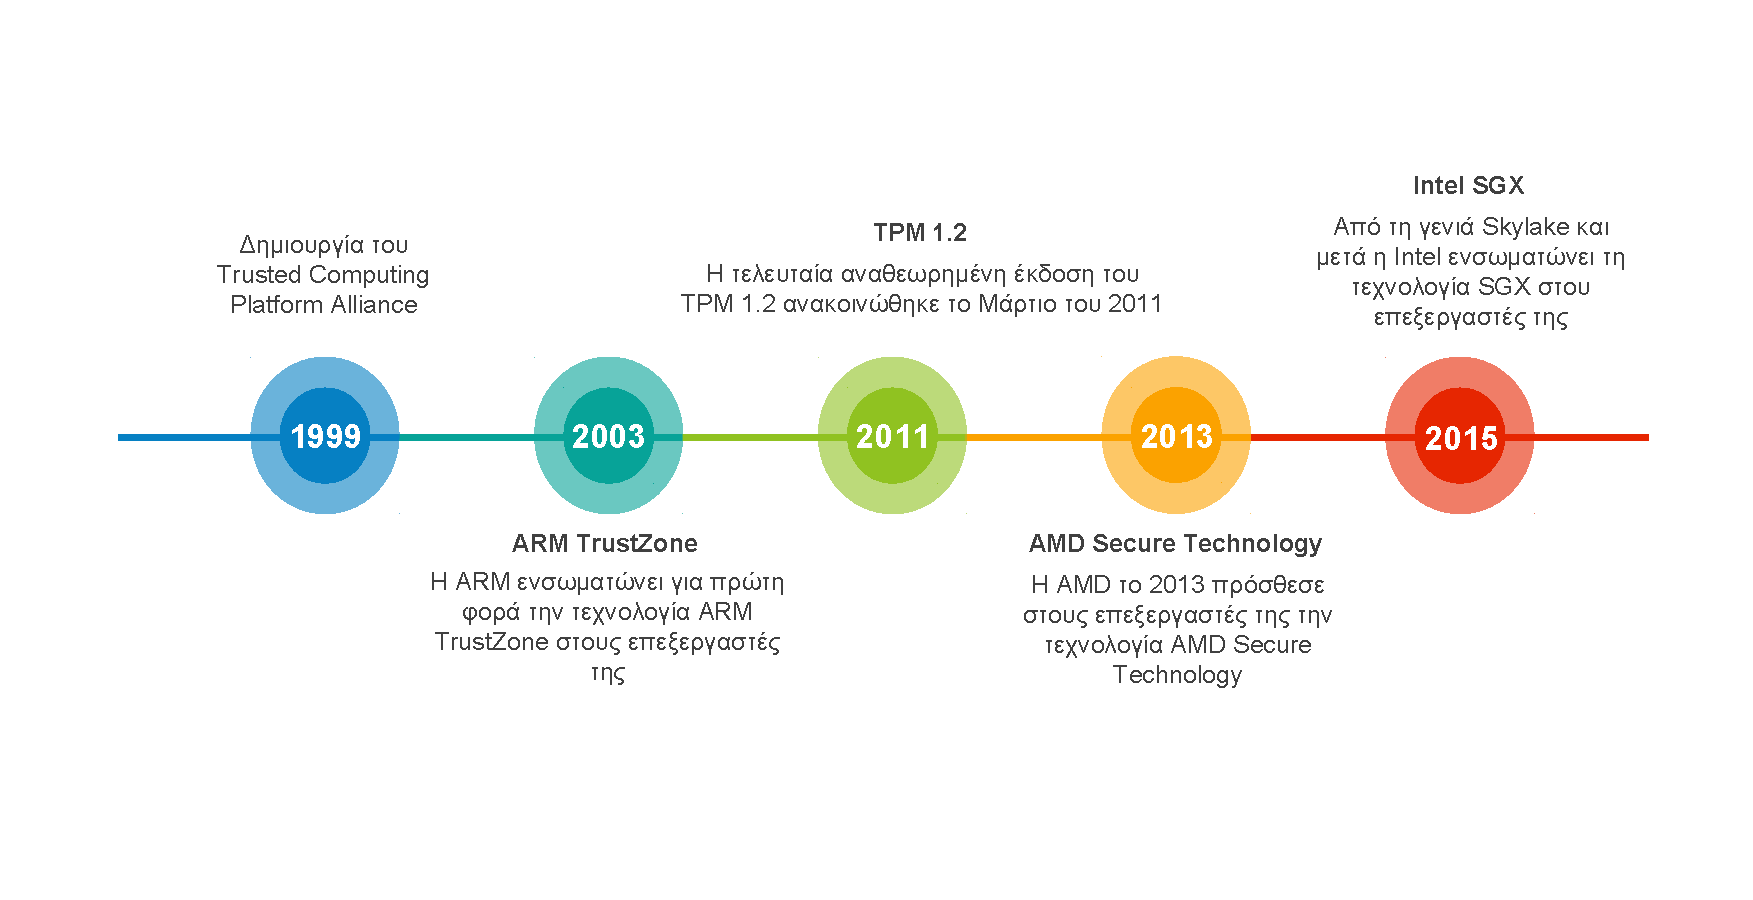
\includegraphics[width=1.3\linewidth]{trusted-hardware-timeline.pdf}
    }
\caption{Ιστορική εξέλιξη των μηχανισμών ασφαλείας υλικού}
\end{figure}


\section{Intel Software Guard Extensions - SGX}
Hello, here is some text without a meaning. This text should show what a printed text
will look like at this place. If you read this text, you will get no information. Really? Is there
no information? Is there a difference between this text and some nonsense like “Huardest
gefburn”? Kjift – not at all! A blind text like this gives you information about the selected
font, how the letters are written and an impression of the look. This text should contain
all letters of the alphabet and it should be written in of the original language. There is no
need for special content, but the length of words should match the language \cite{teeintro}.



\subsection{Enclave}
Αυτό που επιτρέπει στους επεξεργαστές που είναι εξοπλισμένοι με το SGX να παρέχουν αυτές τις ισχυρές εγγυήσεις βασίζεται στα δύο ακόλουθα hardware: Το Processor Reserved Memory (PRM) που είναι ένα συνεχές μπλοκ μνήμης που προορίζεται για το SGX, απρόσιτο από το μη αξιόπιστο λογισμικό και ακόμη και από το υλικό. Η λειτουργία Enclave είναι μια λειτουργία υπό την οποία ένας επεξεργαστής αποκτά πρόσβαση στο PRM.

Αυτό που επιτρέπει στους επεξεργαστές που είναι εξοπλισμένοι με το SGX να παρέχουν αυτές τις ισχυρές εγγυήσεις βασίζεται στα δύο ακόλουθα hardware: Το Processor Reserved Memory (PRM) που είναι ένα συνεχές μπλοκ μνήμης που προορίζεται για το SGX, απρόσιτο από το μη αξιόπιστο λογισμικό και ακόμη και από το υλικό. Η λειτουργία Enclave είναι μια λειτουργία υπό την οποία ένας επεξεργαστής αποκτά πρόσβαση στο PRM.

Αυτό που επιτρέπει στους επεξεργαστές που είναι εξοπλισμένοι με το SGX να παρέχουν αυτές τις ισχυρές εγγυήσεις βασίζεται στα δύο ακόλουθα hardware: Το Processor Reserved Memory (PRM) που είναι ένα συνεχές μπλοκ μνήμης που προορίζεται για το SGX, απρόσιτο από το μη αξιόπιστο λογισμικό και ακόμη και από το υλικό. Η λειτουργία Enclave είναι μια λειτουργία υπό την οποία ένας επεξεργαστής αποκτά πρόσβαση στο PRM.

Αυτό που επιτρέπει στους επεξεργαστές που είναι εξοπλισμένοι με το SGX να παρέχουν αυτές τις ισχυρές εγγυήσεις βασίζεται στα δύο ακόλουθα hardware: Το Processor Reserved Memory (PRM) που είναι ένα συνεχές μπλοκ μνήμης που προορίζεται για το SGX, απρόσιτο από το μη αξιόπιστο λογισμικό και ακόμη και από το υλικό. Η λειτουργία Enclave είναι μια λειτουργία υπό την οποία ένας επεξεργαστής αποκτά πρόσβαση στο PRM.

Αυτό που επιτρέπει στους επεξεργαστές που είναι εξοπλισμένοι με το SGX να παρέχουν αυτές τις ισχυρές εγγυήσεις βασίζεται στα δύο ακόλουθα hardware: Το Processor Reserved Memory (PRM) που είναι ένα συνεχές μπλοκ μνήμης που προορίζεται για το SGX, απρόσιτο από το μη αξιόπιστο λογισμικό και ακόμη και από το υλικό. Η λειτουργία Enclave είναι μια λειτουργία υπό την οποία ένας επεξεργαστής αποκτά πρόσβαση στο PRM.

Αυτό που επιτρέπει στους επεξεργαστές που είναι εξοπλισμένοι με το SGX να παρέχουν αυτές τις ισχυρές εγγυήσεις βασίζεται στα δύο ακόλουθα hardware: Το Processor Reserved Memory (PRM) που είναι ένα συνεχές μπλοκ μνήμης που προορίζεται για το SGX, απρόσιτο από το μη αξιόπιστο λογισμικό και ακόμη και από το υλικό. Η λειτουργία Enclave είναι μια λειτουργία υπό την οποία ένας επεξεργαστής αποκτά πρόσβαση στο PRM.


\begin{figure}[H]
\centering
  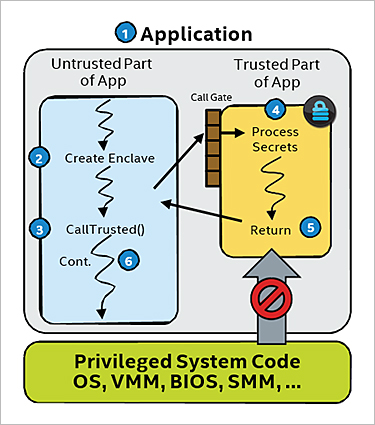
\includegraphics[scale=0.93]{runtime-execution-sgx.png}
  \caption{Τα βήματα που ακολουθούνται στο enclave κατά τη διάρκεια εκτέλεσης. Πηγή: software.intel.com }
  \label{fig:runtime_exetutionsgx}
\end{figure}

\begin{enumerate}
   \item Η εφαρμογή δημιουργείται με trusted και untrusted μέρη
   \item Η εφαρμογή εκτελείται και δημιουργεί το enclave, το οποίο είναι σε ασφαλή απομονωμένη μνήμη
\item Καλείται η trusted μέθοδος και η εκτέλεση μεταφέρεται στο enclave
\item Το enclave βλέπει όλα τα δεδομένα τη διεργασίας, η πρόσβαση από έξω στα δεδομένα του enclave απαγορεύεται.
\item Η trusted function επιστρέφει τα δεδομένα του enclave
\item Η εφαρμογή συνεχίζει την κανονική της εκτέλεση
 \end{enumerate}




\subsection{Attestation}
Αυτό που επιτρέπει στους επεξεργαστές που είναι εξοπλισμένοι με το SGX να παρέχουν αυτές τις ισχυρές εγγυήσεις βασίζεται στα δύο ακόλουθα hardware: Το Processor Reserved Memory (PRM) που είναι ένα συνεχές μπλοκ μνήμης που προορίζεται για το SGX, απρόσιτο από το μη αξιόπιστο λογισμικό και ακόμη και από το υλικό. Η λειτουργία Enclave είναι μια λειτουργία υπό την οποία ένας επεξεργαστής αποκτά πρόσβαση στο PRM.

\subsubsection{Local attestation}

Αυτό που επιτρέπει στους επεξεργαστές που είναι εξοπλισμένοι με το SGX να παρέχουν αυτές τις ισχυρές εγγυήσεις βασίζεται στα δύο ακόλουθα hardware: Το Processor Reserved Memory (PRM) που είναι ένα συνεχές μπλοκ μνήμης που προορίζεται για το SGX, απρόσιτο από το μη αξιόπιστο λογισμικό και ακόμη και από το υλικό. Η λειτουργία Enclave είναι μια λειτουργία υπό την οποία ένας επεξεργαστής αποκτά πρόσβαση στο PRM.

Αυτό που επιτρέπει στους επεξεργαστές που είναι εξοπλισμένοι με το SGX να παρέχουν αυτές τις ισχυρές εγγυήσεις βασίζεται στα δύο ακόλουθα hardware: Το Processor Reserved Memory (PRM) που είναι ένα συνεχές μπλοκ μνήμης που προορίζεται για το SGX, απρόσιτο από το μη αξιόπιστο λογισμικό και ακόμη και από το υλικό. Η λειτουργία Enclave είναι μια λειτουργία υπό την οποία ένας επεξεργαστής αποκτά πρόσβαση στο PRM.

\begin{figure}[H]
\centering
  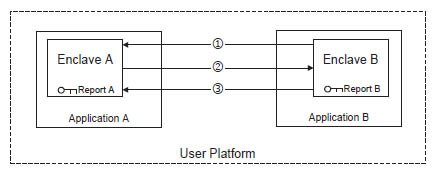
\includegraphics[scale=0.85]{local-attestation-sealing.jpg}
  \caption{Διαδικασία τοπικής βεβαίωσης (Local attestation). Πηγή: software.intel.com }
  \label{fig:runtime_localattestation}
\end{figure}

Το σχήμα \ref{fig:runtime_localattestation} δείχνει ένα παράδειγμα ροής για το πως δύο enclave στην ίδια πλατφόρμα πιστοποιούν το ένα το άλλο. 
\begin{enumerate}
   \item Η εφαρμογή Α έχει το enclave A και η εφαρμογή Β έχει το enclave B. Αφού πρώτα η κάθε εφαρμογή δημιούργησε μια διαδρομή επικοινωνίας με το enclave της, το enclave B στέλνει την ταυτότητα (MRENCLAVE) του στο enclave A.
   \item Το enclave A ζητάει από το hardware να δημιουργήσει μία αναφορά προορισμένη για το enclave B χρησιμοποιώντας το MRENCLAVE που έλαβε από το enclave Β. Το enclave A στέλνει την αναφορά του στο enclave Β μέσω της untrusted εφαρμογής. Σαν μέρος της αναφοράς, το enclave Α μπορεί επίσης να στείλει δεδομένα στον Β.
\item Μόλις λάβει το enclave Β την αναφορά απο το enclave Α, το enclave Β ζητάει από το hardware να πιστοποιήσει την αναφορά για να επιβεβαιώσει το enclave Β ότι το enclave Α είναι στην ίδια πλατφόρμα με αυτό. Το enclave Β μπορεί τώρα να απαντήσει χρησιμοποιώντας την αναφορά του enclave Α, χρησιμοποιώντας την MRENCLAVE τιμή από την αναφορά που μόλις έλαβε. Το enclave B στέλνει την αναφορά του στο enclave A.
\item To enclave A τότε πιστοποιεί την αναφορά για να επιβεβαιωθεί ότι το enclave Β ανήκει στην ίδια πλατφόρμα με το enclave Α.

 \end{enumerate}


\subsubsection{Remote attestation}

Αυτό που επιτρέπει στους επεξεργαστές που είναι εξοπλισμένοι με το SGX να παρέχουν αυτές τις ισχυρές εγγυήσεις βασίζεται στα δύο ακόλουθα hardware: Το Processor Reserved Memory (PRM) που είναι ένα συνεχές μπλοκ μνήμης που προορίζεται για το SGX, απρόσιτο από το μη αξιόπιστο λογισμικό και ακόμη και από το υλικό. Η λειτουργία Enclave είναι μια λειτουργία υπό την οποία ένας επεξεργαστής αποκτά πρόσβαση στο PRM.

Αυτό που επιτρέπει στους επεξεργαστές που είναι εξοπλισμένοι με το SGX να παρέχουν αυτές τις ισχυρές εγγυήσεις βασίζεται στα δύο ακόλουθα hardware: Το Processor Reserved Memory (PRM) που είναι ένα συνεχές μπλοκ μνήμης που προορίζεται για το SGX, απρόσιτο από το μη αξιόπιστο λογισμικό και ακόμη και από το υλικό. Η λειτουργία Enclave είναι μια λειτουργία υπό την οποία ένας επεξεργαστής αποκτά πρόσβαση στο PRM.

\begin{figure}[H]
\centering
  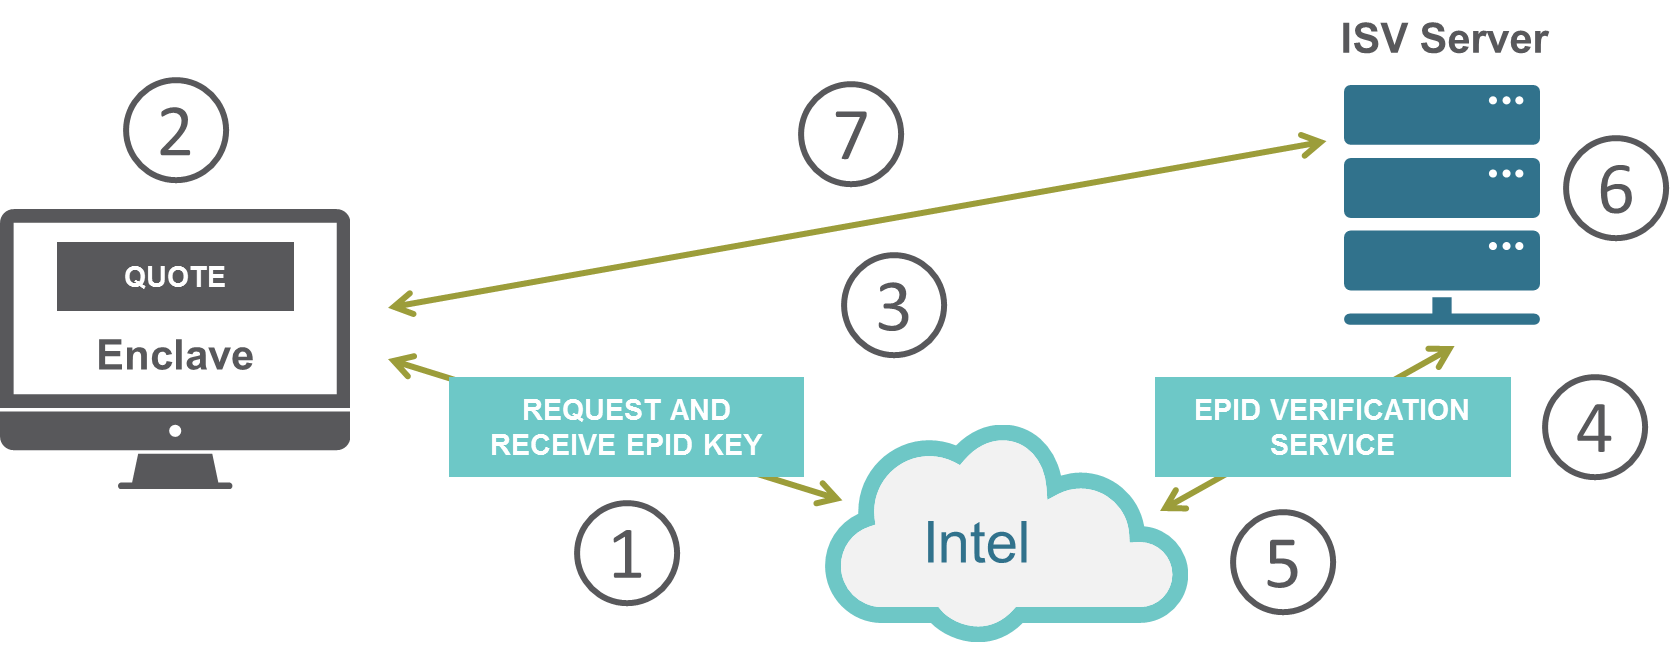
\includegraphics[width=1\linewidth]{remote-sgx.png}
  \caption{Διαδικασία απομακρυσμένης βεβαίωσης (Remote attestation) }
  \label{fig:remote_attestation_sgx}
\end{figure}

\begin{enumerate}
   \item Μετά την εγκατάσταση του λογισμικού Intel SGX Platform (PSW) στον υπολογιστή-πελάτη, το PSW ζητά από την υπηρεσία παροχής υπηρεσιών SGX της Intel να παράσχει το κλειδί EPID (Enhanced Privacy ID) του υπολογιστή. Αν η ανταλλαγή πρωτοκόλλων μεταξύ της υπηρεσίας Intel SGX PSW και της υπηρεσίας παροχής υπηρεσιών Intel είναι επιτυχής - κάτι που απαιτεί γνήσια CPU εξοπλισμένη με Intel SGX, τότε η συσκευή ή ο διακομιστής θα  έχει το κλειδί EPID.
   \item Το enclave παράγει ένα quote. Ένα quote είναι απλώς μια υπογεγραμμένη αναφορά των τρεχουσών τιμών του Platform Configuration Registers (PCRs) στον υπολογιστή. Ο επεξεργαστής του υπολογιστή που τρέχει το enclave δημιουργεί αυτομάτως αυτό το quote.

\item Ο υπολογιστής που τρέχει το enclave στέλνει τότε το quote στον ανεξάρτητο προμηθευτή λογισμικού (Independent software vendor, ISV) που έχει ένα μυστικό που χρειάζεται η εφαρμογή του enclave.

\item O ISV με τη σειρά του στέλνει τo quote στην Intel για επαλήθευση.

\item Η Intel επαληθεύει το quote για τον ISV. Ωστόσο, η Intel δεν παρέχει άλλες πληροφορίες (όπως ποιος δημιούργησε το quote). Στην περίπτωση αυτή, η Intel είναι σαν συμβολαιογράφος: το μόνο που μπορεί να πει είναι ότι το κρυπτογραφικά υπογεγραμμένο quote προέρχεται από έγκυρο enclave, αλλά τίποτα περισσότερο.
\item Στη συνέχεια, ο ISV είναι υπεύθυνος για την επιθεώρηση του quote. Για παράδειγμα, το ISV μπορεί να επιβεβαιώσει ότι το κλειδί είναι δικό του.
\item Αφού ο ISV ικανοποιηθεί με το quote, ο διακομιστής του ISV και το enclave μπορούν τώρα να παράξουν ένα κλειδί κρυπτογράφησης από το quote. Αυτό είναι ένα συμμετρικό κλειδί μεταξύ του διακομιστή και του enclave που χρησιμοποιεί τον αλγόριθμο Diffie-Hellman.
 \end{enumerate}
Αυτό που επιτρέπει στους επεξεργαστές που είναι εξοπλισμένοι με το SGX να παρέχουν αυτές τις ισχυρές εγγυήσεις βασίζεται στα δύο ακόλουθα hardware: Το Processor Reserved Memory (PRM) που είναι ένα συνεχές μπλοκ μνήμης που προορίζεται για το SGX, απρόσιτο από το μη αξιόπιστο λογισμικό και ακόμη και από το υλικό. Η λειτουργία Enclave είναι μια λειτουργία υπό την οποία ένας επεξεργαστής αποκτά πρόσβαση στο PRM.


\subsection{Monotonic counters}
Μία από τις λειτουργίες που παρέχει η Intel SGX, η οποία είναι ιδιαίτερα σημαντική για αυτήν την εργασία, είναι η πρόσβαση σε αξιόπιστους μονοτονικούς μετρητές. Όπως υποδεικνύεται από το όνομα, οι μονοτονικοί μετρητές είναι ακέραιοι μετρητές, οι οποίοι μπορούν μόνο να αυξηθούν.

Μία από τις λειτουργίες που παρέχει η Intel SGX, η οποία είναι ιδιαίτερα σημαντική για αυτήν την εργασία, είναι η πρόσβαση σε αξιόπιστους μονοτονικούς μετρητές. Όπως υποδεικνύεται από το όνομα, οι μονοτονικοί μετρητές είναι ακέραιοι μετρητές, οι οποίοι μπορούν μόνο να αυξηθούν.

Το Intel SGX παρέχει τέσσερις κλήσεις σχετικές με τον μονοτονικό μετρητή:
\begin{itemize}[noitemsep]
\item Η κλήση $sgx\_create\_monotonic\_counter$ δημιουργεί έναν μονοτονικό μετρητή με την προεπιλεγμένη πολιτική κατόχου 0x1, που σημαίνει ότι τα enclaves με το ίδιο κλειδί υπογραφής έχουν πρόσβαση στον μονοτονικό μετρητή.
\item Η κλήση $sgx\_increment\_monotonic\_counter$ αυξάνει την τιμή ενός μετρητή κατά 1.
\item Η κλήση $sgx\_read\_monotonic\_counter$ επιστρέφει την τιμή του μετρητή.
\item Η κλήση $sgx\_destroy\_monotonic\_counter$ καταστρέφει τον μετρητή.
\end{itemize}

\section{Blockchain}
Μία από τις λειτουργίες που παρέχει η Intel SGX, η οποία είναι ιδιαίτερα σημαντική για αυτήν την εργασία, είναι η πρόσβαση σε αξιόπιστους μονοτονικούς μετρητές. Όπως υποδεικνύεται από το όνομα, οι μονοτονικοί μετρητές είναι ακέραιοι μετρητές, οι οποίοι μπορούν μόνο να αυξηθούν.

\subsection{Τι είναι Blockchain}
Ένα blockchain είναι μια ανοιχτή βάση δεδομένων που διατηρεί ένα κατανεμημένο λογιστικό κατάλογο που συνήθως αναπτύσσεται μέσα σε ένα δίκτυο peer-to-peer. Αποτελείτε από μια συνεχώς αυξανόμενη λίστα εγγραφών που ονομάζονται block, τα οποία περιέχουν συναλλαγές. Τα block προστατεύονται από παραβιάσεις με την χρήση κρυπτογραφικών hashes και με μηχανισμό συμφωνίας.

Ένα blockchain είναι μια ανοιχτή βάση δεδομένων που διατηρεί ένα κατανεμημένο λογιστικό κατάλογο που συνήθως αναπτύσσεται μέσα σε ένα δίκτυο peer-to-peer. Αποτελείτε από μια συνεχώς αυξανόμενη λίστα εγγραφών που ονομάζονται block, τα οποία περιέχουν συναλλαγές. Τα block προστατεύονται από παραβιάσεις με την χρήση κρυπτογραφικών hashes και με μηχανισμό συμφωνίας.

Ένα blockchain είναι μια ανοιχτή βάση δεδομένων που διατηρεί ένα κατανεμημένο λογιστικό κατάλογο που συνήθως αναπτύσσεται μέσα σε ένα δίκτυο peer-to-peer. Αποτελείτε από μια συνεχώς αυξανόμενη λίστα εγγραφών που ονομάζονται block, τα οποία περιέχουν συναλλαγές. Τα block προστατεύονται από παραβιάσεις με την χρήση κρυπτογραφικών hashes και με μηχανισμό συμφωνίας.

Ένα blockchain είναι μια ανοιχτή βάση δεδομένων που διατηρεί ένα κατανεμημένο λογιστικό κατάλογο που συνήθως αναπτύσσεται μέσα σε ένα δίκτυο peer-to-peer. Αποτελείτε από μια συνεχώς αυξανόμενη λίστα εγγραφών που ονομάζονται block, τα οποία περιέχουν συναλλαγές. Τα block προστατεύονται από παραβιάσεις με την χρήση κρυπτογραφικών hashes και με μηχανισμό συμφωνίας.

Ένα blockchain είναι μια ανοιχτή βάση δεδομένων που διατηρεί ένα κατανεμημένο λογιστικό κατάλογο που συνήθως αναπτύσσεται μέσα σε ένα δίκτυο peer-to-peer. Αποτελείτε από μια συνεχώς αυξανόμενη λίστα εγγραφών που ονομάζονται block, τα οποία περιέχουν συναλλαγές. Τα block προστατεύονται από παραβιάσεις με την χρήση κρυπτογραφικών hashes και με μηχανισμό συμφωνίας.

\subsection{Το πρωτόκολλο BFT στην τεχνολογία Blockchain}
Η αναπαραγωγή του blockchain πάσχει από βραχυπρόθεσμη ασυνέπεια. Ακόμα κι αν υποθέσουμε άπειρη εκτέλεση και είμαστε πρόθυμοι να υποθέσουμε ότι ένα μπλοκ που είναι θαμμένο από κρυπτογραφικά παζλ αξίας μιας ώρας είναι απολύτως ασφαλές, αυτό σημαίνει ότι πρέπει να περιμένουμε μια ώρα! Στην πραγματικότητα ένα από τα μεγαλύτερα πλεονεκτήματα των πρωτοκόλλων BFT είναι ότι παρέχουν "άμεση οριστικότητα".

Η αναπαραγωγή του blockchain πάσχει από βραχυπρόθεσμη ασυνέπεια. Ακόμα κι αν υποθέσουμε άπειρη εκτέλεση και είμαστε πρόθυμοι να υποθέσουμε ότι ένα μπλοκ που είναι θαμμένο από κρυπτογραφικά παζλ αξίας μιας ώρας είναι απολύτως ασφαλές, αυτό σημαίνει ότι πρέπει να περιμένουμε μια ώρα! Στην πραγματικότητα ένα από τα μεγαλύτερα πλεονεκτήματα των πρωτοκόλλων BFT είναι ότι παρέχουν "άμεση οριστικότητα".


\section{Πρωτόκολλο BFT - Byzantine fault tolerance}
Υπενθυμίζουμε ότι ένα blockchain απαιτεί ένα μηχανισμό για την επίτευξη κατανεμημένης συμφωνίας ή την επικύρωση και την κανονικοποίηση ενός μόνο καταλόγου. Το πρωτόκολλο BFT αναφέρεται στο χαρακτηριστικό των κατανεμημένων συστημάτων που τους επιτρέπει να φτάσουν σε συμφωνία ενάντια στα βυζαντινά σφάλματα, δηλαδή σε καταστάσεις όπου τα συστατικά του συστήματος θα αποτύχουν - αλλά όχι μόνο να αποτύχουν - οι εσφαλμένοι βυζαντινοί κόμβοι θα ενεργήσουν αυθαίρετα και συχνά παρουσιάζουν αντικρουόμενες πληροφορίες σε διαφορετικούς κόμβους του συστήματος.

Οι αλγόριθμοι BFT τυπικά απαιτούν $3f + 1$ servers (ή replicas) για να ανεχθούν $f$ βυζαντινούς (ή ελαττωματικούς) διακομιστές. Βασίζονται στην ιδέα ότι τα σωστά αντίγραφα μπορούν να ξεπεράσουν τα ελαττωματικά αντίγραφα με μια σειρά ψήφων και, για να συμβεί αυτό, θα χρειαστούν τουλάχιστον $2f + 1$ σωστά αντίγραφα, σε σύνολο εξυπηρετητών $3f + 1$. Ωστόσο, αυτοί οι αλγόριθμοι απαιτούν περισσότερους διακομιστές από αυτό το ελάχιστο.

\begin{figure}
  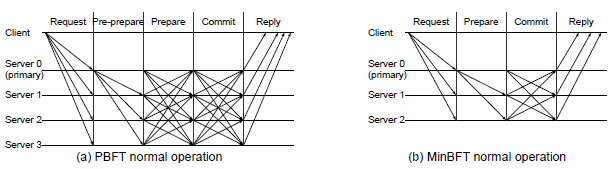
\includegraphics[scale=0.93]{Message-patterns-of-PBFT-and-MinBFT4.png}
  \caption{Ακολουθία μηνυμάτων των PBFT και MinBFT (Figure 1 από \cite{minbftpaper}).}
  \label{fig:minbftpatterns1}
\end{figure}


\section{Practical BFT - PBFT} \label{pbftSection}
Το Practical Byzantine Fault Tolerance (PBFT) είναι ένας αλγόριθμος BFT που δημοσιεύθηκε το 1999 στην εργασία ''Practical Byzantine Fault Tolerance'' \cite{pbft}. Στοχεύει να βελτιώσει τον αυθεντικό BFT μηχανισμό συμφωνίας και υλοποιήθηκε σε πολλά μοντέρνα κατανεμημένα υπολογιστικά συστήματα, συμπεριλαμβανομένων και μερικών γνωστών blockchain. Το PBFT απαιτεί $3f + 1$ servers (ή replicas) για να ανεχθεί $f$ βυζαντινούς (ή ελαττωματικούς) διακομιστές. Ουσιαστικά, όλοι οι κόμβοι του μοντέλου PBFT οργανώνονται σε μια ακολουθία με έναν κόμβο να είναι ο πρωτεύον κόμβος (leader) και οι άλλοι να είναι εφεδρικοί κόμβοι. Όλοι οι κόμβοι του συστήματος επικοινωνούν μεταξύ τους και ο στόχος είναι η επίτευξη συμφωνίας για την κατάσταση του συστήματος μέσω πλειοψηφίας.

\begin{figure}[H]
\centering
  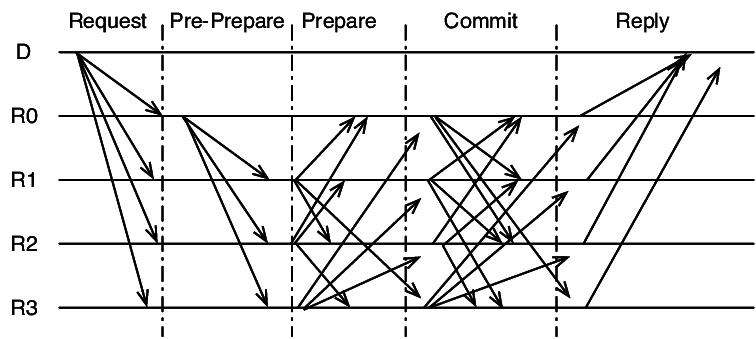
\includegraphics[width=1\linewidth]{The-normal-operation-of-the-PBFT-algorithm.png}
  \caption{Κανονική λειτουργία του PBFT }
  \label{fig:pbft_normal}
\end{figure}

Κάθε γύρος στο PBFT για την επίτευξη συμφωνίας αποτελείτε από 4 φάσεις. Αυτό το μοντέλο είναι περισσότερο «Διοικητή και υποδιοικητή» από ένα καθαρό πρόβλημα βυζαντινών στρατηγών (BFT), όπου όλοι οι στρατηγοί είναι ίσοι, λόγω της παρουσίας ενός κόμβου ηγέτη. Οι φάσεις είναι οι εξής:
\begin{enumerate}
\item Ένας client στέλνει ένα αίτημα στον πρωτεύον διακομιστή.
\item Ο πρωτεύον κόμβος διανέμει το αίτημα στους εφεδρικούς κόμβους.
\item Οι κόμβοι εκτελούν το αίτημα και στη συνέχεια στέλνουν μια απάντηση στον client.
\item Ο client αναμένει $f + 1$ (το f αντιπροσωπεύει το μέγιστο αριθμό κόμβων που ενδέχεται να είναι ελαττωματικοί) από διαφορετικούς κόμβους. 
\end{enumerate}

Οι τρεις φάσεις είναι οι pre-prepare, prepare, και commit. Οι φάσεις pre-prepare και prepare χρησιμοποιούνται για να διατάξουν αιτήματα που στάλθηκαν στον ίδιο γύρο ακόμα και αν ο πρωτεύων διακομιστής είναι ελαττωματικός, που σημαίνει η διάταξη των αιτημάτων είναι λανθασμένη. Οι φάσεις prepare και commit χρησιμοποιούνται για να βεβαιωθεί ότι τα αιτήματα που γίνονται commit είναι πλήρως διατεταγμένα σε κάθε γύρο.

Είναι απαραίτητο οι κόμβοι να είναι ντετερμινιστικοί και να ξεκινούν από τη ίδια κατάσταση. Το τελικό αποτέλεσμα είναι όλοι οι ειλικρινής κόμβοι να έρθουν σε συμφωνία, είτε αποδέχονται είτε απορρίπτουν ένα αίτημα.

\section{MinBFT} \label{minbftSection}
Το MinBFT, είναι ένας $2f + 1$ αλγόριθμος συμφωνίας με βυζαντινά σφάλματα (BFT). O αλγόριθμος MinBFT ακολουθεί ένα πρότυπο ανταλλαγής μηνυμάτων παρόμοιο με το PBFT (βλ. Σχήμα \ref{fig:minbftpatterns1}). Οι διακομιστές οργανώνονται σε ομάδες που ονομάζονται $views$. Κάθε $view$ έχει έναν πρωτεύον διακομιστή και όλοι οι υπόλοιποι είναι εφεδρικά αντίγραφα (backups). Οι clients είναι αυτοί που δημιουργούν τα αιτήματα που ενσωματώνουν κάποιες λειτουργίες για να εκτελεστούν από τους διακομιστές.

Υπενθυμίζουμε ότι ένα blockchain απαιτεί ένα μηχανισμό για την επίτευξη κατανεμημένης συμφωνίας ή την επικύρωση και την κανονικοποίηση ενός μόνο καταλόγου. Το πρωτόκολλο BFT αναφέρεται στο χαρακτηριστικό των κατανεμημένων συστημάτων που τους επιτρέπει να φτάσουν σε συμφωνία ενάντια στα βυζαντινά σφάλματα, δηλαδή σε καταστάσεις όπου τα συστατικά του συστήματος θα αποτύχουν - αλλά όχι μόνο να αποτύχουν - οι εσφαλμένοι βυζαντινοί κόμβοι θα ενεργήσουν αυθαίρετα και συχνά παρουσιάζουν αντικρουόμενες πληροφορίες σε διαφορετικούς κόμβους του συστήματος.

Υπενθυμίζουμε ότι ένα blockchain απαιτεί ένα μηχανισμό για την επίτευξη κατανεμημένης συμφωνίας ή την επικύρωση και την κανονικοποίηση ενός μόνο καταλόγου. Το πρωτόκολλο BFT αναφέρεται στο χαρακτηριστικό των κατανεμημένων συστημάτων που τους επιτρέπει να φτάσουν σε συμφωνία ενάντια στα βυζαντινά σφάλματα, δηλαδή σε καταστάσεις όπου τα συστατικά του συστήματος θα αποτύχουν - αλλά όχι μόνο να αποτύχουν - οι εσφαλμένοι βυζαντινοί κόμβοι θα ενεργήσουν αυθαίρετα και συχνά παρουσιάζουν αντικρουόμενες πληροφορίες σε διαφορετικούς κόμβους του συστήματος.


\textbf{Clients}. Ένας client $c$ για να ζητήσει την εκτέλεση μιας λειτουργίας $op$ στέλνει ένα μήνυμα της μορφής $<$REQUEST, c, seq, op$>\sigma_{c}$ σε όλους τους διακομιστές. Ο αριθμός $seq$ είναι ο αναγνωριστικός κωδικός της αίτησης που χρησιμοποιείται για να εξασφαλιστεί η μοναδικότητα. Οι διακομιστές αποθηκεύουν σε ένα πίνακα $V_{req}$ τον αριθμό $seq$ του τελευταίου αιτήματος που έχουν εκτελέσει για κάθε πελάτη, απορρίπτουν αιτήματα με αναγνωριστικό κωδικό $seq$ μικρότερο από το τελευταίο εκτελεσμένο (για να αποφευχθεί η εκτέλεση του ίδιου αιτήματος δύο φορές) και τέλος τυχόν αιτήματα που λαμβάνονται όσο το προηγούμενο είναι υπό επεξεργασία. Τα αιτήματα υπογράφονται με το ιδιωτικό κλειδί του client και αιτήματα με μη έγκυρη υπογραφή $c$ απλά απορρίπτονται. Μετά από την αποστολή ενός αιτήματος, ο client περιμένει για $f + 1$ απαντήσεις της μορφής $<$REPLY, s, seq, res$>$ από διαφορετικούς διακομιστές $s$ με αντίστοιχα αποτελέσματα $res$, γεγονός που εξασφαλίζει ότι τουλάχιστον μία απάντηση θα προέρχεται από σωστό διακομιστή. Στην περίπτωση που ο client δεν λάβει αρκετές απαντήσεις κατά τη διάρκεια ενός χρονικού διαστήματος που διαβάζεται από το τοπικό ρολόι του, ξαναστέλνει το αίτημα. Σε περίπτωση που το αίτημα αυτό έχει ήδη υποβληθεί σε επεξεργασία, οι διακομιστές θα ξαναστείλουν την αποθηκευμένη απάντηση τους.

\textbf{Διακομιστές}. Υπενθυμίζουμε ότι ένα blockchain απαιτεί ένα μηχανισμό για την επίτευξη κατανεμημένης συμφωνίας ή την επικύρωση και την κανονικοποίηση ενός μόνο καταλόγου. Το πρωτόκολλο BFT αναφέρεται στο χαρακτηριστικό των κατανεμημένων συστημάτων που τους επιτρέπει να φτάσουν σε συμφωνία ενάντια στα βυζαντινά σφάλματα, δηλαδή σε καταστάσεις όπου τα συστατικά του συστήματος θα αποτύχουν - αλλά όχι μόνο να αποτύχουν - οι εσφαλμένοι βυζαντινοί κόμβοι θα ενεργήσουν αυθαίρετα και συχνά παρουσιάζουν αντικρουόμενες πληροφορίες σε διαφορετικούς κόμβους του συστήματος.

Η ιδέα είναι ότι ένα αίτημα $m$ στέλνεται από το πρωτεύον διακομιστή $s_{i}$ σε όλους τους διακομιστές σε ένα μήνυμα τύπου $<PREPARE, v, s_{i}, m, UI_{i}>$, και κάθε server $s_{j}$ το ξαναστέλνει σε όλους τους άλλους σε ένα μήνυμα τύπου $<COMMIT, v, s_{j}, s_{i},m, UI_{i},$ $UI_{j}>$, όπου το $UI_{j}$ λαμβάνεται καλώντας το $createUI$. Κάθε μήνυμα που αποστέλλεται, είτε είναι $PREPARE$ είτε $COMMIT$, έχει ως εκ τούτου ένα μοναδικό αναγνωστικό $UI$ που αποκτάται καλώντας τη συνάρτηση $createUI$, έτσι ώστε να μην υπάρχουν δύο μηνύματα με το ίδιο αναγνωριστικό. Οι διακομιστές ελέγχουν εάν τα αναγνωριστικά των μηνυμάτων που λαμβάνουν ισχύουν για αυτά τα μηνύματα, χρησιμοποιώντας μια λειτουργία επαλήθευσης.

Στην περίπτωση που ένας διακομιστής $s_{k}$ δεν έλαβε κάποιο μήνυμα PREPARE αλλά έλαβε ένα μήνυμα COMMIT με έγκυρο αναγνωριστικό, τότε στέλνει το δικό του COMMIT. Αυτό μπορεί να συμβεί αν ο αποστολέας είναι ελαττωματικός και δεν στέλνει το μήνυμα PREPARE στον server $s_{k}$ (αλλά το στέλνει σε άλλους διακομιστές) ή εάν το μήνυμα PREPARE απλώς καθυστερεί και λαμβάνεται μετά τα μηνύματα COMMIT. Ένα αίτημα $m$ γίνεται αποδεκτό από έναν διακομιστή που εκτελεί τον αλγόριθμο εάν ο διακομιστής λάβει $f + 1$ έγκυρα μηνύματα $COMMIT$ από διαφορετικούς διακομιστές για το αίτημα $m$.

Υπενθυμίζουμε ότι ένα blockchain απαιτεί ένα μηχανισμό για την επίτευξη κατανεμημένης συμφωνίας ή την επικύρωση και την κανονικοποίηση ενός μόνο καταλόγου. Το πρωτόκολλο BFT αναφέρεται στο χαρακτηριστικό των κατανεμημένων συστημάτων που τους επιτρέπει να φτάσουν σε συμφωνία ενάντια στα βυζαντινά σφάλματα, δηλαδή σε καταστάσεις όπου τα συστατικά του συστήματος θα αποτύχουν - αλλά όχι μόνο να αποτύχουν - οι εσφαλμένοι βυζαντινοί κόμβοι θα ενεργήσουν αυθαίρετα και συχνά παρουσιάζουν αντικρουόμενες πληροφορίες σε διαφορετικούς κόμβους του συστήματος.

Υπενθυμίζουμε ότι ένα blockchain απαιτεί ένα μηχανισμό για την επίτευξη κατανεμημένης συμφωνίας ή την επικύρωση και την κανονικοποίηση ενός μόνο καταλόγου. Το πρωτόκολλο BFT αναφέρεται στο χαρακτηριστικό των κατανεμημένων συστημάτων που τους επιτρέπει να φτάσουν σε συμφωνία ενάντια στα βυζαντινά σφάλματα, δηλαδή σε καταστάσεις όπου τα συστατικά του συστήματος θα αποτύχουν - αλλά όχι μόνο να αποτύχουν - οι εσφαλμένοι βυζαντινοί κόμβοι θα ενεργήσουν αυθαίρετα και συχνά παρουσιάζουν αντικρουόμενες πληροφορίες σε διαφορετικούς κόμβους του συστήματος.

Υπενθυμίζουμε ότι ένα blockchain απαιτεί ένα μηχανισμό για την επίτευξη κατανεμημένης συμφωνίας ή την επικύρωση και την κανονικοποίηση ενός μόνο καταλόγου. Το πρωτόκολλο BFT αναφέρεται στο χαρακτηριστικό των κατανεμημένων συστημάτων που τους επιτρέπει να φτάσουν σε συμφωνία ενάντια στα βυζαντινά σφάλματα, δηλαδή σε καταστάσεις όπου τα συστατικά του συστήματος θα αποτύχουν - αλλά όχι μόνο να αποτύχουν - οι εσφαλμένοι βυζαντινοί κόμβοι θα ενεργήσουν αυθαίρετα και συχνά παρουσιάζουν αντικρουόμενες πληροφορίες σε διαφορετικούς κόμβους του συστήματος.

\section{Η υπηρεσία USIG} \label{usigSection}
Υπενθυμίζουμε ότι ένα blockchain απαιτεί ένα μηχανισμό για την επίτευξη κατανεμημένης συμφωνίας ή την επικύρωση και την κανονικοποίηση ενός μόνο καταλόγου. Το πρωτόκολλο BFT αναφέρεται στο χαρακτηριστικό των κατανεμημένων συστημάτων που τους επιτρέπει να φτάσουν σε συμφωνία ενάντια στα βυζαντινά σφάλματα, δηλαδή σε καταστάσεις όπου τα συστατικά του συστήματος θα αποτύχουν - αλλά όχι μόνο να αποτύχουν - οι εσφαλμένοι βυζαντινοί κόμβοι θα ενεργήσουν αυθαίρετα και συχνά παρουσιάζουν αντικρουόμενες πληροφορίες σε διαφορετικούς κόμβους του συστήματος.
Το interface της υπηρεσίας έχει δύο λειτουργίες: 
\begin{itemize}
\item createUI ($m$) - επιστρέφει ένα πιστοποιητικό USIG που περιέχει ένα μοναδικό αναγνωριστικό $UI$ και πιστοποιεί ότι αυτό το $UI$ δημιουργήθηκε από την αξιόπιστη και απαραβίαστη μονάδα για το μήνυμα $m$. Το μοναδικό αναγνωριστικό είναι ουσιαστικά μια ανάγνωση του μονοτονικού μετρητή, ο οποίος αυξάνεται κάθε φορά που καλείται η $createUI$. 
\item verifyUI ($PK$, $UI$, $m$) - επαληθεύει εάν το μοναδικό αναγνωριστικό $UI$ είναι έγκυρο για το μήνυμα $m$, δηλαδή εάν το πιστοποιητικό USIG ταιριάζει με το μήνυμα και τα υπόλοιπα δεδομένα στο $UI$.
\end{itemize}

Υπενθυμίζουμε ότι ένα blockchain απαιτεί ένα μηχανισμό για την επίτευξη κατανεμημένης συμφωνίας ή την επικύρωση και την κανονικοποίηση ενός μόνο καταλόγου. Το πρωτόκολλο BFT αναφέρεται στο χαρακτηριστικό των κατανεμημένων συστημάτων που τους επιτρέπει να φτάσουν σε συμφωνία ενάντια στα βυζαντινά σφάλματα, δηλαδή σε καταστάσεις όπου τα συστατικά του συστήματος θα αποτύχουν - αλλά όχι μόνο να αποτύχουν - οι εσφαλμένοι βυζαντινοί κόμβοι θα ενεργήσουν αυθαίρετα και συχνά παρουσιάζουν αντικρουόμενες πληροφορίες σε διαφορετικούς κόμβους του συστήματος.

\section{Σύγκριση με άλλες ερευνητικές εργασίες}
Υπενθυμίζουμε ότι ένα blockchain απαιτεί ένα μηχανισμό για την επίτευξη κατανεμημένης συμφωνίας ή την επικύρωση και την κανονικοποίηση ενός μόνο καταλόγου. Το πρωτόκολλο BFT αναφέρεται στο χαρακτηριστικό των κατανεμημένων συστημάτων που τους επιτρέπει να φτάσουν σε συμφωνία ενάντια στα βυζαντινά σφάλματα, δηλαδή σε καταστάσεις όπου τα συστατικά του συστήματος θα αποτύχουν - αλλά όχι μόνο να αποτύχουν - οι εσφαλμένοι βυζαντινοί κόμβοι θα ενεργήσουν αυθαίρετα και συχνά παρουσιάζουν αντικρουόμενες πληροφορίες σε διαφορετικούς κόμβους του συστήματος.


%Hybster
\begin{figure}[H]
 \centering
  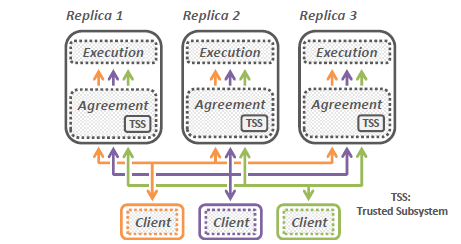
\includegraphics[scale=0.93]{Message-pattern-in-HybSter1.png}
  \caption{Hybrid BFT state-machine replication (Figure 1 από \cite{hybster})}
  \label{fig:hybster1}
\end{figure}

\begin{figure}[H]
 \centering
  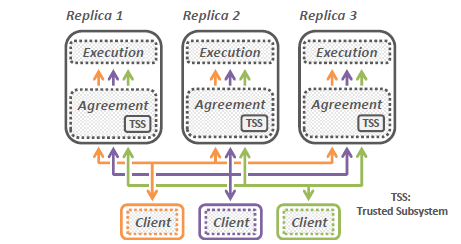
\includegraphics[scale=0.93]{Message-pattern-in-HybSter1.png}
  \caption{Η ιδέα της παραλληλοποίησης του υβριδικού πρωτοκόλλου (Figure 2 από \cite{hybster})}
  \label{fig:hybster2}
\end{figure}

Υπενθυμίζουμε ότι ένα blockchain απαιτεί ένα μηχανισμό για την επίτευξη κατανεμημένης συμφωνίας ή την επικύρωση και την κανονικοποίηση ενός μόνο καταλόγου. Το πρωτόκολλο BFT αναφέρεται στο χαρακτηριστικό των κατανεμημένων συστημάτων που τους επιτρέπει να φτάσουν σε συμφωνία ενάντια στα βυζαντινά σφάλματα, δηλαδή σε καταστάσεις όπου τα συστατικά του συστήματος θα αποτύχουν - αλλά όχι μόνο να αποτύχουν - οι εσφαλμένοι βυζαντινοί κόμβοι θα ενεργήσουν αυθαίρετα και συχνά παρουσιάζουν αντικρουόμενες πληροφορίες σε διαφορετικούς κόμβους του συστήματος.

%CheapBFT

\begin{figure}[H]
 \centering
  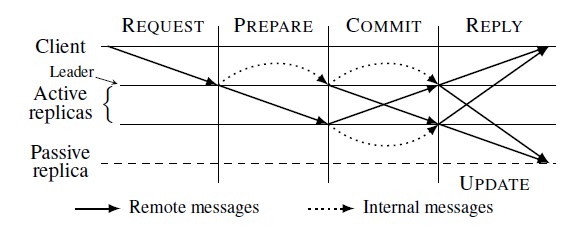
\includegraphics[scale=0.93]{Message-pattern-in-CheapBFT.jpg}
  \caption{Ακολουθία μηνυμάτων του CheapBFT (Figure 4 από \cite{cheapbft}).}
  \label{fig:cheapbftpatterns1}
\end{figure}

Υπενθυμίζουμε ότι ένα blockchain απαιτεί ένα μηχανισμό για την επίτευξη κατανεμημένης συμφωνίας ή την επικύρωση και την κανονικοποίηση ενός μόνο καταλόγου. Το πρωτόκολλο BFT αναφέρεται στο χαρακτηριστικό των κατανεμημένων συστημάτων που τους επιτρέπει να φτάσουν σε συμφωνία ενάντια στα βυζαντινά σφάλματα, δηλαδή σε καταστάσεις όπου τα συστατικά του συστήματος θα αποτύχουν - αλλά όχι μόνο να αποτύχουν - οι εσφαλμένοι βυζαντινοί κόμβοι θα ενεργήσουν αυθαίρετα και συχνά παρουσιάζουν αντικρουόμενες πληροφορίες σε διαφορετικούς κόμβους του συστήματος.

%FastBFT
\begin{figure}[H]
 \centering
  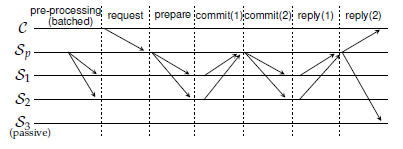
\includegraphics[scale=0.93]{Message-pattern-in-FastBFT.png}
  \caption{Ακολουθία μηνυμάτων του FastBFT (Figure 2 από \cite{fastbft}).}
  \label{fig:fastbftpatterns1}
\end{figure}

Ομοίως, το FastBFT \cite{fastbft} Υπενθυμίζουμε ότι ένα blockchain απαιτεί ένα μηχανισμό για την επίτευξη κατανεμημένης συμφωνίας ή την επικύρωση και την κανονικοποίηση ενός μόνο καταλόγου. Το πρωτόκολλο BFT αναφέρεται στο χαρακτηριστικό των κατανεμημένων συστημάτων που τους επιτρέπει να φτάσουν σε συμφωνία ενάντια στα βυζαντινά σφάλματα, δηλαδή σε καταστάσεις όπου τα συστατικά του συστήματος θα αποτύχουν - αλλά όχι μόνο να αποτύχουν - οι εσφαλμένοι βυζαντινοί κόμβοι θα ενεργήσουν αυθαίρετα και συχνά παρουσιάζουν αντικρουόμενες πληροφορίες σε διαφορετικούς κόμβους του συστήματος.
